% ---------------------------------------------------------------
% Preamble
% ---------------------------------------------------------------
\documentclass[a4paper,11pt]{article}

\usepackage[utf8]{inputenc}
\usepackage[english]{babel}
\usepackage[margin=1in,a4paper,pdftex]{geometry}
\usepackage[protrusion=true,expansion=true]{microtype} 
\usepackage{amsmath,amsfonts,amsthm,amssymb,bm,mathdots,mathtools,bigints}
\usepackage{rotating}
\usepackage[colorlinks=true, linkcolor=blue, urlcolor=blue, anchorcolor=blue, citecolor=red]{hyperref}
\usepackage[all]{hypcap}
\usepackage{color, xcolor}
\usepackage{listings}
\usepackage[ruled,linesnumbered]{algorithm2e}
\usepackage{cite}
\usepackage{makecell}
\usepackage[printwatermark]{xwatermark}
\usepackage{subcaption}
\usepackage{siunitx}
\usepackage{tikz, pgfplots}

\usepackage{framed}
\definecolor{myYellow}{rgb}{1,0.65,0}
\definecolor{myRed}{rgb}{0.84, 0.18, 0.13}
\definecolor{myGreen}{rgb}{0, 0.53, 0.27}
\definecolor{myBlue}{rgb}{0, 0.34, 0.91}
\colorlet{shadecolor}{myBlue!7}

\numberwithin{figure}{section}
\numberwithin{equation}{section}
\numberwithin{table}{section}

\newtheorem{theorem}{Theorem}[section]
\newtheorem{corollary}{Corollary}[theorem]
\newtheorem{lemma}[theorem]{Lemma}

\theoremstyle{definition}
\newtheorem{definition}{Definition}[section]

%\newwatermark[allpages,color=red!15,angle=45,scale=5,xpos=-1cm,ypos=2cm]{DRAFT}

\makeatletter
\setlength{\@fptop}{0pt}
\makeatother

\usepackage{graphicx}
\graphicspath{ {figs/} }

\newbox{\bigpicturebox}

\lstset{
    backgroundcolor=\color[rgb]{0.86,0.88,0.93},
    language=matlab, keywordstyle=\color[rgb]{0,0,1},
    basicstyle=\footnotesize \ttfamily,breaklines=true,
    escapeinside={\%*}{*)}
}

% --------------------------------------------------------------------
% Tikz Macros
% --------------------------------------------------------------------
\usetikzlibrary{shapes,arrows, backgrounds, positioning, fit, decorations.pathmorphing}

\tikzstyle{sectionBlock} = [draw, fill=blue!20, rectangle, minimum height=3em, minimum width=3em]
\tikzstyle{block} = [draw, fill=white, rectangle, minimum height=3em, minimum width=3em]
\tikzstyle{sum} = [draw, fill=white, circle, node distance=1cm]
\tikzstyle{input} = [coordinate]
\tikzstyle{output} = [coordinate]
\tikzstyle{pinstyle} = [pin edge={to-,thin,black}]
\tikzstyle{mcInput} = [draw, rectangle, line width=0.5mm, minimum width=2em, minimum height=2em, fill=black!10]
\tikzstyle{mcCircle} = [draw, circle, line width=0.5mm, minimum width=2em, minimum height=2em, fill=white]

% --------------------------------------------------------------------
% Definitions
% --------------------------------------------------------------------
\newcommand{\HRule}[1]{\rule{\linewidth}{#1}} 

\makeatletter                       
\def\printtitle{
    {\centering \@title\par}}
\makeatother                                    

\makeatletter 
\def\printauthor{
    {\centering \large \@author}}               
\makeatother                            

\newcounter{boxed-theorem}
\makeatletter
\newenvironment{boxed-theorem}[1]
{\begin{shaded} \begin{theorem}{#1}}
{\end{theorem} \end{shaded}}

\newcounter{boxed-definition}
\makeatletter
\newenvironment{boxed-definition}[1]
{\begin{shaded} \begin{definition}{#1}}
{\end{definition} \end{shaded}}

% ---------------------------------------------------------------
% Metadata 
% ---------------------------------------------------------------
\title{ \normalsize \textsc{TI0119 - PROCESSAMENTO DIGITAL DE SINAIS} 
        \\[2.0cm]             
        \HRule{0.5pt} \\              
        \LARGE \textbf{\uppercase{Projeto de Filtros Digitais}\\2º Exerc\'icio Computacional}
        \HRule{2pt} \\[0.5cm]  
}

\author{
        Otacílio Bezerra Leite Neto\\   
        Universidade Federal do Ceará\\  
        Departamento de Engenharia de Teleinform\'atica\\
        \texttt{minhotmog@gmail.com} \\
}

\begin{document}
% ---------------------------------------------------------------
% Maketitle
% ---------------------------------------------------------------
\thispagestyle{empty}       % Remove page numbering on this page

\printtitle                 % Print the title data as defined above
    \vfill
\printauthor                % Print the author data as defined above
\newpage

% ---------------------------------------------------------------
% Begin document
% ---------------------------------------------------------------
\setcounter{secnumdepth}{1}
\setcounter{tocdepth}{1}

% 1 - Introduction
% ---------------------------------------------------------------
\clearpage
\setcounter{page}{1}
\section{Projeto de Filtro Butterworth}

Neste documento apresenta-se o procedimento para o projeto de um Filtro Digital do tipo IIR (Infinite Impulse Response) utilizando dois métodos distintos: \textit{Invariância do Impulso} e \textit{Trasnformação Bilinear}. Um filtro de passa-baixa é um dispositivo designado a manter  componentes de frequência de um sinal antes de uma certa \textit{frequência de corte}. Da mesma forma, esse filtro deve "rejeitar" as componentes de frequência desse sinal a partir dessa mesma frequência. Uma vez que um filtro ideal é impraticável, trabalha-se com filtros que realizem uma filtragem dado as especificações digitais tais como indicadas na Figura abaixo.

\vskip0.3cm
\noindent \begin{minipage}{\textwidth} \centering
	\begin{minipage}{0.49\textwidth}
		\centering
		\includegraphics[width=\textwidth]{lowpass.png}
	\end{minipage}
	\hfill
	\begin{minipage}{0.49\textwidth}
		\begin{tabular}{c l}
			\textbf{Legenda} &  \\
			\hline
			$\omega_p$ & Frequência máxima (\textit{Passband}) \\
			$\omega_s$ & Frequência mínima (\textit{Stopband}) \\
			$\delta_{p1}$ & \makecell{Limite superior de variação\\(\textit{Passband})} \\
			$\delta_{p2}$ & \makecell{Limite inferior de variação\\(\textit{Passband})} \\
			$\delta_{s}$ & \makecell{Limite superior de variação\\(\textit{Stopband})}
		\end{tabular}
	\end{minipage}
\end{minipage}
\vskip0.3cm

Nesse trabalho, tratamos especificamente do Filtro de Butterworth, cuja função de transferência analógica é representada no formato:
\begin{equation} \label{eq:butter}
    H_c(s) = \frac{K}{\displaystyle\prod_{i=0}^{N-1} \left( s - \Omega_c e^{j\left( \frac{\pi(1+2k+N)}{2N} \right)} \right)}	
,\end{equation}

\noindent onde o ganho $K = \lim_{s \to 0} \texttt{den}(H_c(s))$, e os parâmetros $\Omega_c$ e $N$ são, respectivamente, a \textbf{frequência de corte} e a \textbf{ordem} do filtro. O procedimento para obter o filtro digital, $H(z)$, consiste em obter os parâmetros do filtro análogico e então convertê-lo para a forma digital, utilizando um dos métodos mencionados. O procedimento para cada método é detalhado abaixo.

\subsection{Invariância do Impulso}

Por esse método, consideramos que a resposta do filtro digital para um impulso é obtida através de amostras discretas da resposta ao impulso do filtro analógico. Ou seja,
\begin{equation}
	h[n] = T_d h_c(n T_d),
\end{equation}

\noindent onde $T_d$ representa o tempo de amostragem. Com o método de invariância do impulso, então, teremos a seguinte relação entre as especificações e os parâmetros do Filtro de Butterworth:
\begin{equation} \label{eq:impulse}
\begin{matrix}
	N = \left\lceil \cfrac{1}{2} \cfrac{log \left(\frac{1}{(1-\delta_{p2})^2} - 1 \right) - log \left( \frac{1}{(\delta_{s})^2} - 1 \right)}{log(\omega_p) - log(\omega_s)} \right\rceil; & & 
	\Omega_c = \cfrac{\omega_p}{10^{\frac{1}{2N} log \left(\frac{1}{(1-\delta_{p2})^2} - 1 \right)}}
\end{matrix}
\end{equation}

Com esses parâmetros, podemos utilizar a Função de Transferência em \eqref{eq:butter} e, após uma expansão por frações parciais, converter para a versão digital através da fórmula:
\begin{equation} \label{eq:impulse2}
	H(z) = \sum_{i=0}^{N-1} \cfrac{A_i}{1 - e^{s_i} z^{-1}}
,\end{equation}

\noindent onde
\begin{equation} 
\begin{matrix}
	s_i = \Omega_c e^{j\left( \frac{\pi(1+2i+N)}{2N} \right)}; & A_i = \displaystyle\lim_{s \to s_i} H_c(s) = \cfrac{K}{\displaystyle\prod_{\substack{j = 0 \\ j \neq i}}^{N-1} (s - s_j) }
\end{matrix}
\end{equation}

\subsection{Transformação Bilinear}

Para o método de Transformação Bilinear, o filtro digital é obtido diretamente através do filtro análogico simplesmente ao aplicar a transformação:
\begin{equation} \label{eq:bil_trans}
	s = 2\cfrac{1 - z^{-1}}{1 + z^{-1}} \rightarrow H(z) = H_c \left( 2\cfrac{1 - z^{-1}}{1 + z^{-1}} \right)
\end{equation}

Substituindo $z = e^{j\omega}$, é possível obter a relação
\begin{equation}
	s = \alpha + j \Omega = \cfrac{2j}{T_d}tan(\omega / 2)
\end{equation}

\noindent que diretamente resultam em $\Omega = 2 tan(\omega / 2)$, assumindo $T_d = 1$. Dessa forma, os parâmetros do filtro analógico são obtidos de forma semelhante ao método da Invariância de Impulso, mas transformando as frequências $\Omega_p = 2 tan(\omega_p / 2)$ e $\Omega_s = 2 tan(\omega_s / 2)$ tal que:
\begin{equation} \label{eq:bilinear}
\begin{matrix}
	N = \left\lceil \cfrac{1}{2} \cfrac{log \left(\frac{1}{(1-\delta_{p2})^2} - 1 \right) - log \left( \frac{1}{(\delta_{s})^2} - 1 \right)}{log(tan(\omega_p / 2)) - log(tan(\omega_s / 2))} \right\rceil; & & 
	\Omega_c = \cfrac{2 tan(\omega_s / 2)}{10^{\frac{1}{2N} log \left(\frac{1}{(\delta_{s})^2} - 1 \right)}}
\end{matrix}
.\end{equation}

%% -------------------
\section{Realização de Filtros Analógicos}

Dado uma função de transferência de um Filtro Analógico, é sempre possível obter e implementar o sistema físico equivalente na forma de um circuito elétrico. A síntese de um circuito RLC para um filtro de passa-baixa pode ser realizado ao transformar a função de transferência do filtro,
\begin{equation}
	H_c(s) = \cfrac{1}{\alpha_n s^n + \alpha_{n-1} s^{n-1} + \cdots + \alpha_2 s^2 + \alpha_1 s + \alpha_0},
\end{equation}

\noindent no formato em cascata de
\begin{equation}
	Z_1 = \cfrac{1}{Y_1 + \cfrac{1}{Z_2 + \cfrac{1}{Y_3 + \cdots \cfrac{1}{Z_{n-1} + \cfrac{1}{Y_n + 1/R_L}}}}},
\end{equation}

\noindent do qual $Y_i$ e $Z_j$ são a transformada de Laplace dos capacitores e indutores $C_i$ e $L_i$, respectivamente, dispostos na topologia série-paralela indicada na figura abaixo. Um resistor de resistência $R_L$, não mostrado no diagrama, também é conectado nos terminais do último capacitor, e é nos seus terminais que se afere a tensão resultante do circuito. Nessa topologia, temos a possibilidade de adicionar um resistor no início do circuito para representar o ganho do sistema.

\begin{figure}[ht] \centering
	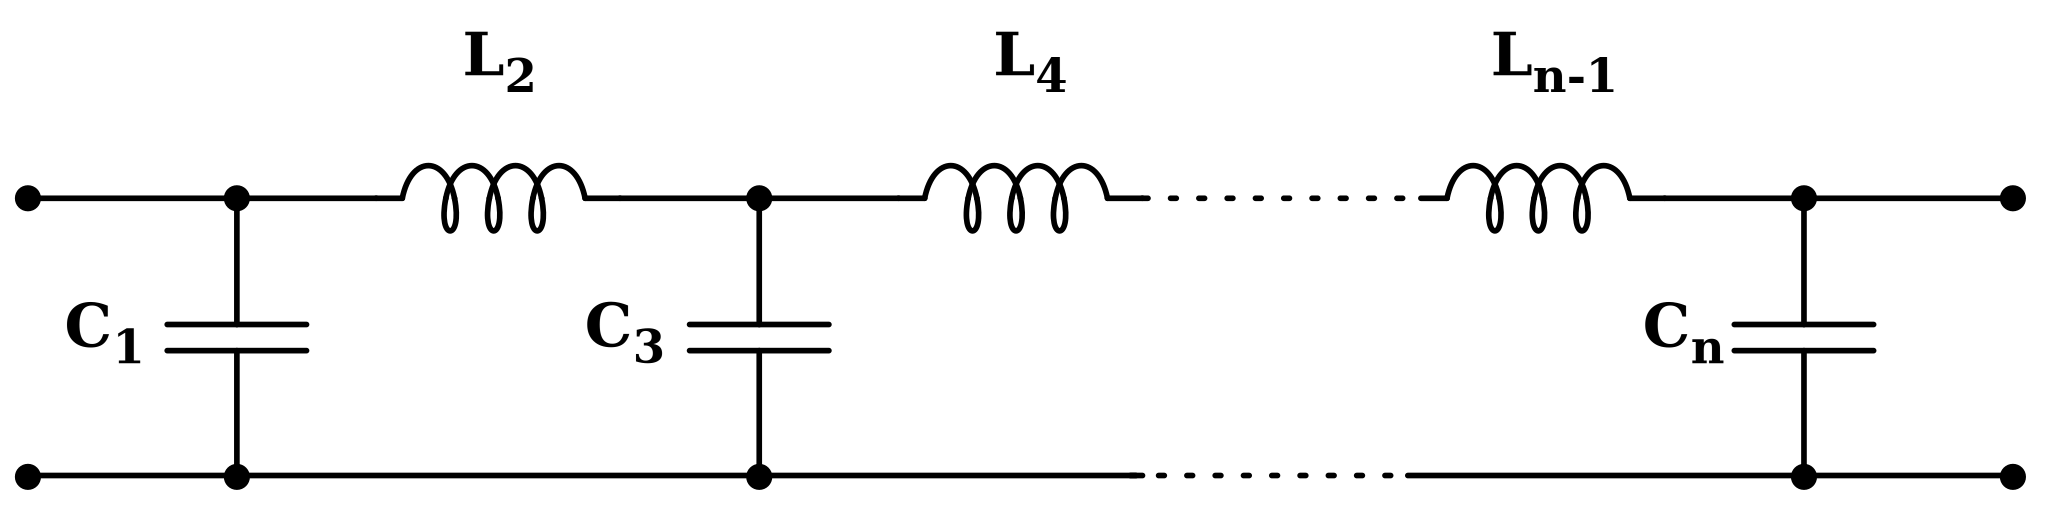
\includegraphics[width=0.72\textwidth]{ladder}
	\caption{Topologia de Cauer, ou topologia \textit{Ladder Network}.}
\end{figure}

%% ---------
\section{Resultados}

Abaixo são demonstrados os resultados para aplicação dos métodos apresentados anteriormente para o projeto e síntese de um filtro passa-baixa do tipo IIR através de um Filtro de Butterworth. O filtro foi projeto para alcançar as especificações:
\begin{equation}
\begin{cases}
0.99 \leq | H(e^{j\omega}) | \leq 1 & \text{se } \phantom{.4\pi}0 \leq |\omega| \leq 0.4\pi \\
\phantom{0.99 \leq\ }| H(e^{j\omega}) | \leq 0.001 & \text{se } 0.6\pi \leq |\omega| \leq \pi
\end{cases}
\end{equation}

\subsection{Invariância do Impulso}

Primeiramente, aplicamos a técnica da Invariância do Impulso para obter os parâmetros do filtro analógico. Utilizando as fórmulas em \eqref{eq:impulse}, teremos que:
\begin{equation}
\begin{matrix}
	N = \left\lceil \cfrac{1}{2} \cfrac{log \left(\frac{1}{(0.99)^2} - 1 \right) - log \left( \frac{1}{(0.001)^2} - 1 \right)}{log(0.4\pi) - log(0.6\pi)} \right\rceil; & & 
	\Omega_c = \cfrac{0.4\pi}{10^{\frac{1}{2N} log \left(\frac{1}{(0.99)^2} - 1 \right)}}
\end{matrix},
\end{equation}

\noindent que então resultam em $N = 22$ e $\Omega_c = 1.373$. 

\subsection{Transformação Bilinear}

No caso da técnica de Transformação Bilinear, realizamos uma transformação não-linear das variáveis de frequência. Utilizando as fórmulas em \eqref{eq:bilinear}, teremos que:
\begin{equation}
\begin{matrix}
	N = \left\lceil \cfrac{1}{2} \cfrac{log \left(\frac{1}{(0.99)^2} - 1 \right) - log \left( \frac{1}{(0.001)^2} - 1 \right)}{log(tan(0.2\pi)) - log(tan(0.3\pi))} \right\rceil; & & 
	\Omega_c = \cfrac{tan(0.3\pi)}{10^{\frac{1}{2N} log \left(\frac{1}{(0.001)^2} - 1 \right)}}
\end{matrix},
\end{equation}

\noindent que então resultam em $N = 14$ e $\Omega_c = 1.681$. 

\subsection{Visualização da Resposta em Frequência}

Uma vez que os parâmetros do filtro analógico são determinados, é possível realizar uma simulação da resposta do filtro, no domínio da frequência. Primeiramente, realizamos a simulação do sistema analógico dos dois filtros obtidos, utilizando a fórmula em \eqref{eq:butter}. O resultado é demonstrado abaixo, analisando a magnitude em decibéis dessa resposta.

\begin{figure}[ht] \centering
	\includegraphics[width=\textwidth]{analog}
	\caption{Resposta em frequência para as duas realizações do Filtro Analógico de Butterworth.}
	\label{fig:analog}
\end{figure}

Podemos perceber que, dado a clara diferença entre os parâmetros obtidos pelos dois métodos, a resposta em frequência do filtro também demonstra uma clara diferença. No caso analógico, o filtro obtido pelo método da invariância exibe um decaimento mais acelerado após determinada frequência, quando comparado com o filtro obtido por transformação bilinear.

Para o filtro digital, que consiste no foco do projeto, a resposta em frequência é obtida utilizando a fórmula em \eqref{eq:impulse2}, no caso do método de Invariância do Impulso, e utilizando o filtro analógico com a transformação de entrada dada por \ref{eq:bil_trans}, no caso do método de Transformação Bilinear. Os dois resultados são expostos abaixo. 

\begin{figure}[ht] \centering
	\includegraphics[width=\textwidth]{digital}
	\caption{Resposta em frequência para as duas realizações do Filtro Digital IIR.}
	\label{fig:digital}
\end{figure}

Nessa visualização, as frequências $\omega_p$ e $\omega_s$ são representadas pelas duas linhas vermelhas tracejadas, indicando a separação entre as bandas de passagem, banda de transição e banda de rejeição, respectivamente. Os limites superiores $\delta_{p2}$ e $\delta_s$, por sua vez, são representados pelas linhas vermelhas pontilhadas. Podemos perceber que ambas as realizações do filtro demonstraram o comportamento de filtragem passa-baixa esperado. Adicionalmente, é possível observar que o filtro obtido pelo método de Transformação Bilinear, nesse caso, demonstrou um decaimento mais rápido na banda de rejeição quando comparado ao método de Invariância de Impulso, portanto demonstrando uma melhor performance nesse contexto.

\subsection{Realização do Filtro Analógico}

Finalmente, demonstramos a realização do Filtro Analógico de Butterworth para a função de transferência determinada pelo método de Transformação Bilinear. Para a composição do circuito elétrico utilizamos a Topologia de Cauer (ou topologia \textit{Ladder Network}), para a qual o circuito RLC equivalente possui a estrutura indicada pela figura abaixo:

\begin{figure}[ht] \centering
	\includegraphics[width=0.86\textwidth]{butterworth}
	\caption{Circuito elétrico analógico para o Filtro de Butterworth.}
	\label{fig:butterworth}
\end{figure}

% ---------------------------------------------------------------
% End document
% ---------------------------------------------------------------

\end{document}

%%%%%%%%%%%%%%%%%%%%%%%%%%%%%%%%%%%
%% Drafts:
%%%%%%%%%%%%%%%%%%%%%%%%%%%%%%%%%%%
%%%%% Figure:
% \begin{figure}[ht]
%   \centering
%   \includegraphics[trim={0cm 0cm 0cm 0cm},clip,scale=1]{nameFigure}
%   \caption{Caption of the figure.}
%   \label{fig:nameFigure}
% \end{figure} \vskip0.25cm
%
%%%%% Equation:
% \begin{equation} \label{eq:nameEquation}
% \begin{split}
%    X = 1 + 1
% \end{split}
% \end{equation} \vskip0.25cm
%
%%%% Table:
% \begin{table}[hp]
%   \centering
%   \begin{tabular}{l | c c }
%   Principal & Coluna1 & Coluna2 \\
%   \hline 
%   ABC & 1 & 2 \\
%   DFG & 3 & 4 \\
%   HIJ & 5 & 6 \\
%   \end{tabular} 
%   \caption{Caption of the table.}
%   \label{table:nameTable} 
% \end{table} \vskip0.25cm

%\begin{figure}
%    \centering
%    \begin{minipage}[t][6cm][t]{.48\textwidth}
%	\begin{tikzpicture}
%	  \begin{axis}[enlargelimits=false, scale only axis, axis on top, width=0.8\textwidth,
%	  	xlabel={$u$ unemployment}, ylabel={$\pi$ inflation}]]
%		\addplot graphics [xmin=0,xmax=96,ymin=0,ymax=96] {chapter3/report_ch3_1_1};
%	  \end{axis}
%	 \end{tikzpicture}
%	\end{minipage}%
%	\hfill
%	\begin{minipage}[t][6cm][t]{0.48\textwidth}
%	\begin{tikzpicture}
%	  \begin{axis}[enlargelimits=false, scale only axis, axis on top, width=0.8\textwidth,
%	  	ylabel={$\pi$ inflation}]]
%		\addplot graphics [xmin=0,xmax=96,ymin=0,ymax=96] {chapter3/report_ch3_1_2};
%	  \end{axis}
%	\end{tikzpicture}%
%	\vspace{.6ex}
%	\begin{tikzpicture}
%		\begin{axis}[enlargelimits=false, scale only axis, axis on top, width=0.8\textwidth,
%	  	xlabel={$u$ unemployment}, ylabel={$\pi$ inflation}]]
%		\addplot graphics [xmin=0,xmax=96,ymin=0,ymax=96] {chapter3/report_ch3_1_3};
%		\end{axis}
%	\end{tikzpicture}
%	\end{minipage}%	
%    
%    \caption{A}
%    \label{fig:regulator01}
%\end{figure}